Thank you for this comment. We agree with you and the referees that spatial spillovers could be a concern in our setting. Although the original manuscript already included a brief spillover check, we appreciate Reviewer 2's suggestion to expand this analysis and provide much stronger reassurance that spillovers do not bias our estimates. We have therefore added a new subsection in the main text and a new appendix with detailed discussion of each exercise. Taken together, the new evidence shows that \emph{Plan Cuadrante} did not displace crime to neighboring municipalities or divert police resources from control to treated areas. We discuss the four exercises below and provide the new manuscript sections.

The first exercise relies on administrative data on reported crime, arrests, and police resources. Since these records are available for all municipalities in the country, we can study what happened around all the municipalities that adopted \emph{Plan Cuadrante} in the period we analyze. Building on our main specification but defining the outcome at the neighboring municipality level, we show that the adoption of \emph{Plan Cuadrante} neither displaced crime from treated to nearby control municipalities nor diverted resources from control to treated areas, both of which would lead us to overestimate the program's effects. These results hold both in the universe of municipalities observed in the administrative records and in the ENUSC subsample in which we study victimization, crime perception, and household investment in security measures.

Second, following the suggestions of Reviewer 2, we implemented variations of the methods developed in \citet{crepon2013} and \citet{Blattman}. In the spirit of \citet{crepon2013}, we estimate the effect of a higher share of neighboring municipalities adopting \emph{Plan Cuadrante} on crime, arrests, and resources in control municipalities, finding no significant effects on any of these outcomes. Next, following \citet{Blattman}, we conduct a randomization inference exercise in which treatment status and adoption dates are randomly assigned 1,000 times, constructing placebo distributions of treatment and spillover effects. The true treatment effect on crime falls in the bottom 1\% of the placebo distribution, while the estimated spillover effects fall within the 40th--45th percentile of the placebo distribution, providing no evidence of meaningful spillovers on crime, arrests, or resources onto neighboring untreated municipalities.

The exercises described in the previous paragraph rely on administrative records from the police, which are available for all municipalities adopting \emph{Plan Cuadrante} in the period we study and for all of their neighboring municipalities. This broad coverage allows us to estimate spillovers credibly using the full set of administrative outcomes. By contrast, outcomes measured in ENUSC are observed for only 46 adopting municipalities and 1 never-treated municipality. This makes spillover analyses more challenging, because coverage of neighboring municipalities is limited: only 10 of these municipalities share a border with another municipality surveyed in ENUSC, and only 6 share a border with either a never-treated municipality or a treated municipality that adopted the program in a different year. Given this limited coverage, the \citet{crepon2013} and \citet{Blattman} exercises are implemented only on the administrative outcomes, for which coverage of neighboring municipalities is sufficient. For the outcomes measured only in ENUSC, we instead estimate the spillover effects of early-adopting ENUSC municipalities on their late-adopting ENUSC neighbors before the latter's own adoption, and once again find no evidence of spatial spillovers.

Below, we provide the sections we added to the updated manuscript:

\textbf{Spatial Spillovers Section:} the new section on spatial spillovers reads as follows:\\
\textbf{4.2 \emph{Plan Cuadrante} and Spatial Spillovers}
\\[12pt]
\begin{adjustwidth}{2em}{0em}
%\textbf{4.2 \emph{Plan Cuadrante} and Spatial Spillovers}

Beyond parallel trends, a causal interpretation of our estimates requires the absence of spillover effects from treated to control municipalities, since such spillovers could bias treatment effects upward. This concern is relevant in our setting. Previous work on deployment-based policing reforms, such as hot-spot policing, shows that crime may be displaced to nearby areas \citep{Blattman_Tobon_JEEA}. Spillovers could also arise through the reallocation of police resources from control to treated municipalities.

In our setting, spillovers are less likely for several reasons. First, as discussed in Section \ref{institutions}, \emph{Plan Cuadrante} introduced beat policing in Chile by reorganizing deployment across the full municipal territory rather than concentrating resources in specific hot spots. Second, Chilean municipalities are large---on average 101,000 inhabitants and 2,000 square kilometers \citep{SINIM}---and criminals typically do not travel such long distances to commit crimes, which makes displacement to other municipalities unlikely \citep{Langella}. Third, and more directly related to police resources, police regulations assign officers to \emph{comisar\'ias}---broader operational units that usually cover an entire municipality---for fixed periods, which limits rapid reallocation of officers across jurisdictions.\footnote{See the Transfer Manual for Carabineros de Chile Personnel available at \url{https://www.carabineros.cl/transparencia/og/pdf/OG_2707_13112019.pdf}}

We nonetheless assess spillovers empirically through two complementary exercises using administrative data at the national level. Online Appendix \ref{sec:appendixC} reports the full results. First, following \citet{crepon2013}, we test whether higher exposure to \emph{Plan Cuadrante} among neighboring municipalities affects outcomes in control municipalities. Online Appendix Figures \ref{fig:figure_continuous_spillovers} and \ref{fig:figure_count_spillovers}---which define neighbor exposure as the share and the number of treated neighbors, respectively---show no meaningful effects across the outcomes we study, suggesting the absence of spatial spillovers. Because exposure to treated neighbors is not randomly assigned, however, this evidence does not fully rule out the possibility that municipalities with many early-adopting neighbors differ systematically from those with fewer such neighbors in other respects that are also correlated with our outcomes.

Second, we estimate the effect of \emph{Plan Cuadrante} on police-reported crime and police resources in untreated municipalities whose neighbors adopt the program. Online Appendix Figure \ref{fig:spillover_admin} summarizes these estimates and again shows no evidence of spatial spillovers.

The exercises above evaluate spatial spillovers using administrative records for the extended municipality sample. We complement this evidence with two additional analyses focused on ENUSC municipalities. First, we re-estimate the administrative-outcome spillover analysis---for reported crime, arrests, police officers, and patrol vehicles---restricting the sample to neighbors of the 46 ENUSC municipalities (Online Appendix Figure \ref{fig:figure_46ENUSC_spillovers_admin}). Second, we test for spillovers directly in ENUSC outcomes. Because ENUSC coverage is limited---46 treated municipalities and 1 never-treated municipality, with only 10 sharing a border and 6 of those treated in different years---we estimate spillover effects from early-adopting ENUSC municipalities onto late-adopting ENUSC neighbors before the latter adopt the program (Online Appendix Figure \ref{fig:figure_results_spillovers_enusc}). Both exercises yield reassuringly null effects.

Taken together, these results indicate that spatial spillovers are unlikely to threaten identification in our setting.

\FloatBarrier
\end{adjustwidth}

\textbf{Spatial Spillovers Appendix:} the new Online Appendix C.9. reads as follows:\\
\textbf{C.9 Testing for Spatial Spillovers}
\\[12pt]
\begin{adjustwidth}{2em}{0em}
This Online Appendix details the specifications behind the spillover tests summarized in Section~\ref{sec:spillovers}.

The baseline test estimates the effect of \emph{Plan Cuadrante} on reported crime, arrests, police officers, and patrol vehicles in neighboring untreated municipalities,
\begin{equation}
Outcome_{mt}= \delta_{1}\,\mbox{\textit{Plan Cuadrante near municip.}}_{mt} + Municipality_{m} + Year_{t} + u_{mt}
\label{eq:main3}
\end{equation}
\noindent where the sample is restricted to municipalities that never adopted the program, each is assigned a treatment date equal to the earliest adoption among its treated neighbors, and $\delta_{1}$ is estimated dynamically with the staggered difference-in-differences estimator of \citet{Callaway}. Because these administrative outcomes are observed for every municipality, we estimate the specification on the full national sample of never treated municipalities (Online Appendix Figure~\ref{fig:spillover_admin}).

For the intensity-based test in the spirit of \citet{crepon2013}, we replace the binary neighbor-treatment indicator with a continuous measure of exposure and restrict the sample to never-treated municipalities,
\begin{equation}
Outcome_{mt}= \delta_{1}\,\mbox{\textit{Share neighbors with Plan Cuadrante}}_{mt} + Municipality_{m} + Year_{t} + u_{mt}
\label{eq:crepon}
\end{equation}
\noindent Because the treatment is continuous, we estimate it with the heterogeneity-robust estimator of \citet{Chaisemartin}, measuring exposure both as the share of treated neighbors (Online Appendix Figure~\ref{fig:figure_continuous_spillovers}) and as their number (Online Appendix Figure~\ref{fig:figure_count_spillovers}).

For the randomization-inference test, we reassign adoption dates and never-treated status across municipalities $1{,}000$ times and re-estimate the direct and spillover effects under the sharp null, yielding the placebo distributions in Online Appendix Figure~\ref{fig:ri_placebo}. For this exercise we rely on the estimator of \citet{Chaisemartin} rather than that of \citet{Callaway}: re-estimating the latter over a thousand permutations would require prohibitive computational power and running time.

Finally, we re-estimate the baseline administrative specification on the municipalities neighboring the 46 ENUSC municipalities (Online Appendix Figure~\ref{fig:figure_46ENUSC_spillovers_admin}); and, for the outcomes measured only in ENUSC, we estimate the spillover of early-adopting ENUSC municipalities on their late-adopting ENUSC neighbors before the latter's own adoption (Online Appendix Figure~\ref{fig:figure_results_spillovers_enusc}). The six focal late-adopters, each shown with its earliest-adopting ENUSC neighbor and that neighbor's adoption year, are Molina (Curic\'o, 2005), Tocopilla (Iquique, 2005), San Carlos (Chill\'an, 2007), Padre Hurtado (Pe\~naflor, 2008), Calera (Quillota, 2008), and Limache (Quillota, 2008). Across all of these specifications, the estimated spillover effects are small and statistically indistinguishable from zero.

\end{adjustwidth}

\clearpage
\noindent\textbf{Other figures and tables referenced above:}
\vspace{0.5em}

{\renewcommand{\thefigure}{C.12}
%--- Implementation
\begin{figure}[h!]
    \centering
    \caption{Geographic Spillovers of \emph{Plan Cuadrante} on Neighboring Untreated Municipalities}
    \label{fig:spillover_admin}
    \begin{subfigure}{0.495\textwidth}
        \centering
        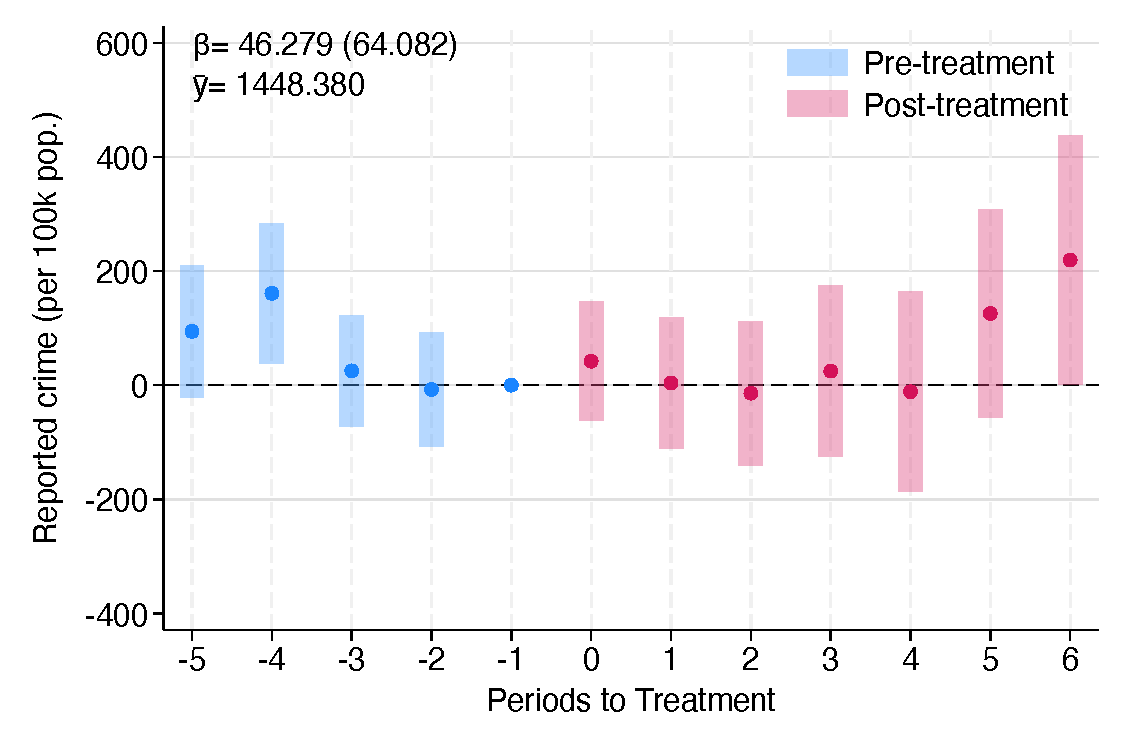
\includegraphics[width=0.98\textwidth]{../manuscript/Graphs/totalreportedcrime_allcomunas_neighbors.pdf}
        \caption{Spillovers on Reported crime}
    \end{subfigure}%
    ~ 
    \begin{subfigure}{0.495\textwidth}
    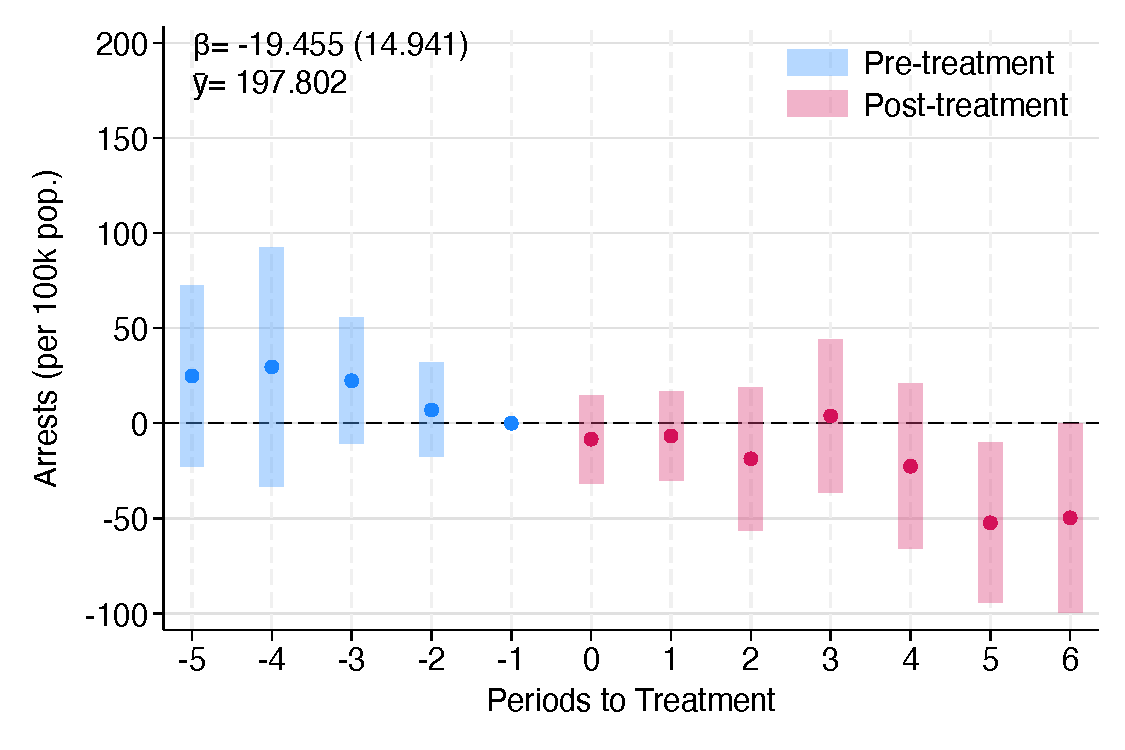
\includegraphics[width=0.98\textwidth]{../manuscript/Graphs/totalarrestscrime_allcomunas_neighbors.pdf}
        \caption{Spillovers on Arrests}
    \end{subfigure}
    \begin{subfigure}{0.495\textwidth}
        \centering
        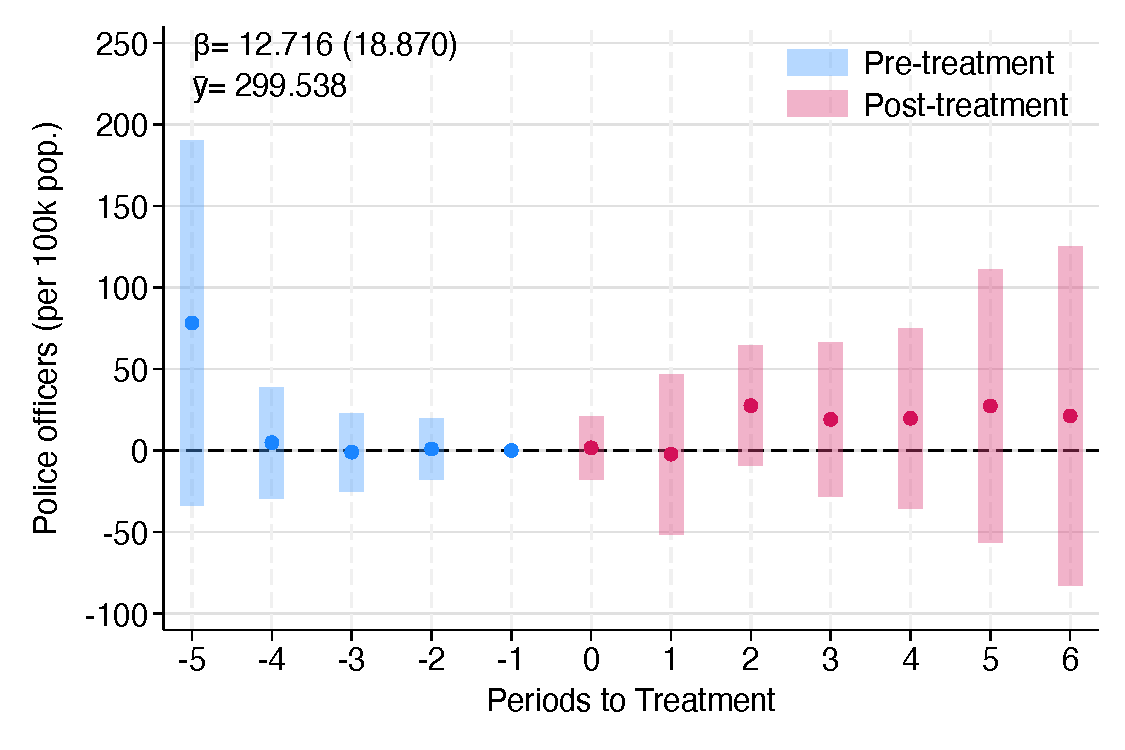
\includegraphics[width=0.98\textwidth]{../manuscript/Graphs/dotpc_allcomunas_neighbors.pdf}
        \caption{Spillovers on Police Officers}
    \end{subfigure}%
    ~ 
    \begin{subfigure}{0.495\textwidth}
    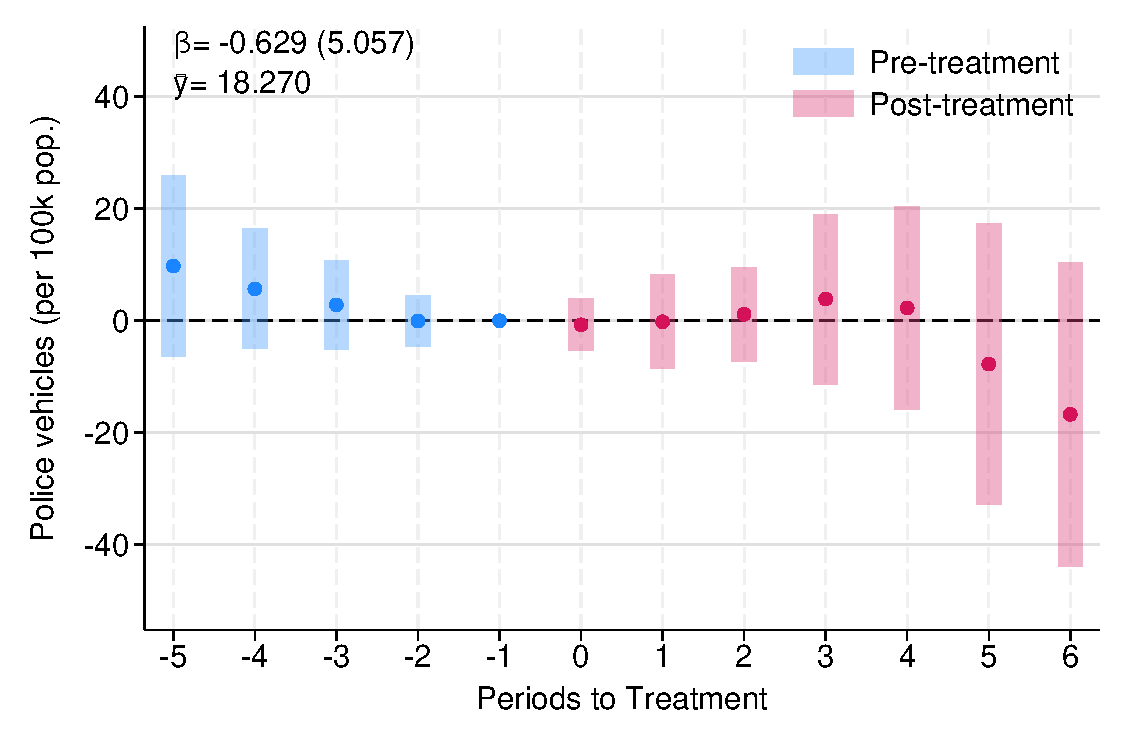
\includegraphics[width=0.98\textwidth]{../manuscript/Graphs/vehiclespc_allcomunas_neighbors.pdf}
        \caption{Spillovers on Patrol Vehicles}
    \end{subfigure}
    \begin{minipage}{0.9\textwidth}
    \footnotesize
    Notes: This figure reports the spillover effects of \emph{Plan Cuadrante} on the number of crimes reported to the police in the municipality per 100,000 inhabitants (panel a), the number of arrests in the municipality per 100,000 inhabitants (panel b), the number of police officers per 100,000 inhabitants (panel c), and the number of patrol vehicles per 100,000 inhabitants (panel d). Panels (a)--(d) include 2,859, 2,166, 1,144, and 1,942 observations respectively. Specifically, the figure shows the dynamic effects of the \emph{Plan Cuadrante} for neighbor municipalities which never introduced the program. The estimation is conducted using the procedure developed in \citet{Callaway} for difference-in-differences with staggered treatment adoption, using as the treatment introduction date the earliest date of a neighboring municipality. The dots in the figure represent the estimated coefficients and the bars behind them 95\% confidence intervals. Standard errors are clustered at the municipality level using the wild bootstrapping procedure. The pooled effect and the mean outcome before the introduction of the treatment for every outcome is also presented in each panel. 
    \end{minipage}
\end{figure}
}

\clearpage

{\setcounter{figure}{12}\renewcommand{\thefigure}{C.\arabic{figure}}
\begin{figure}[h!]
    \centering
    \caption{Geographic Spillovers of \emph{Plan Cuadrante} by Share of Treated Neighbors}
    \label{fig:figure_continuous_spillovers}
    \begin{subfigure}{0.495\textwidth}
        \centering
        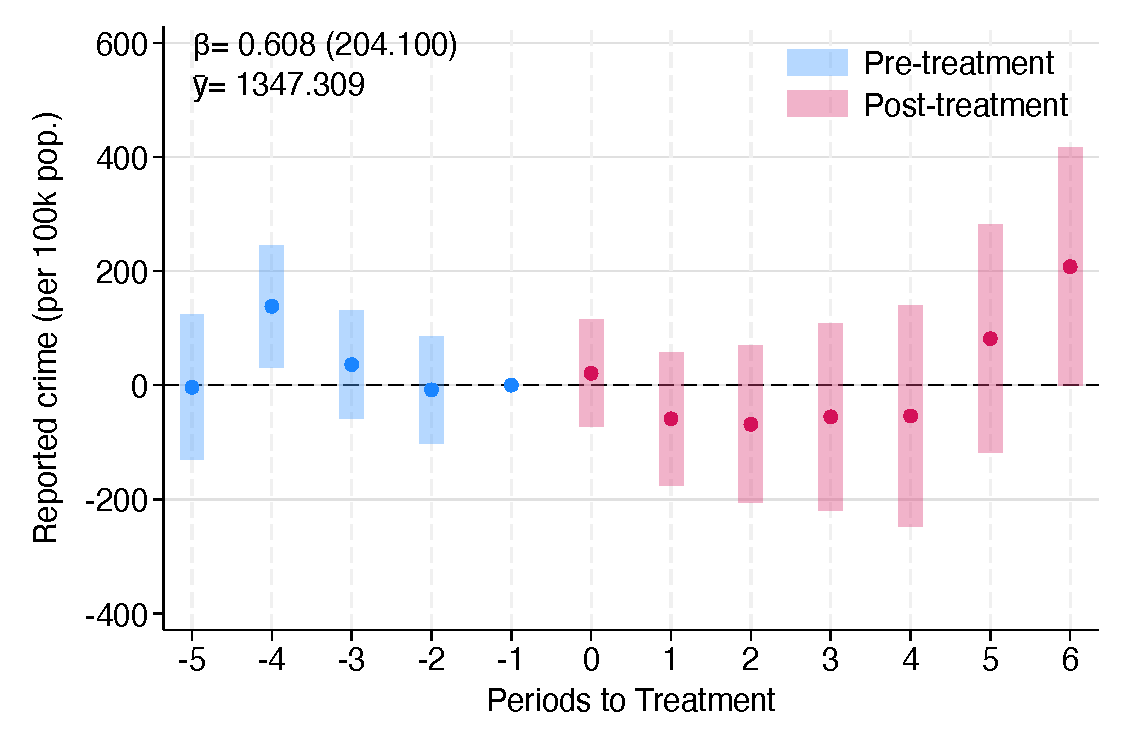
\includegraphics[width=0.98\textwidth]{../manuscript/Graphs/CHDH_continuous_spillover_crime.pdf}
        \caption{Spillovers on Reported Crime}
    \end{subfigure}%
    ~
    \begin{subfigure}{0.495\textwidth}
        \centering
        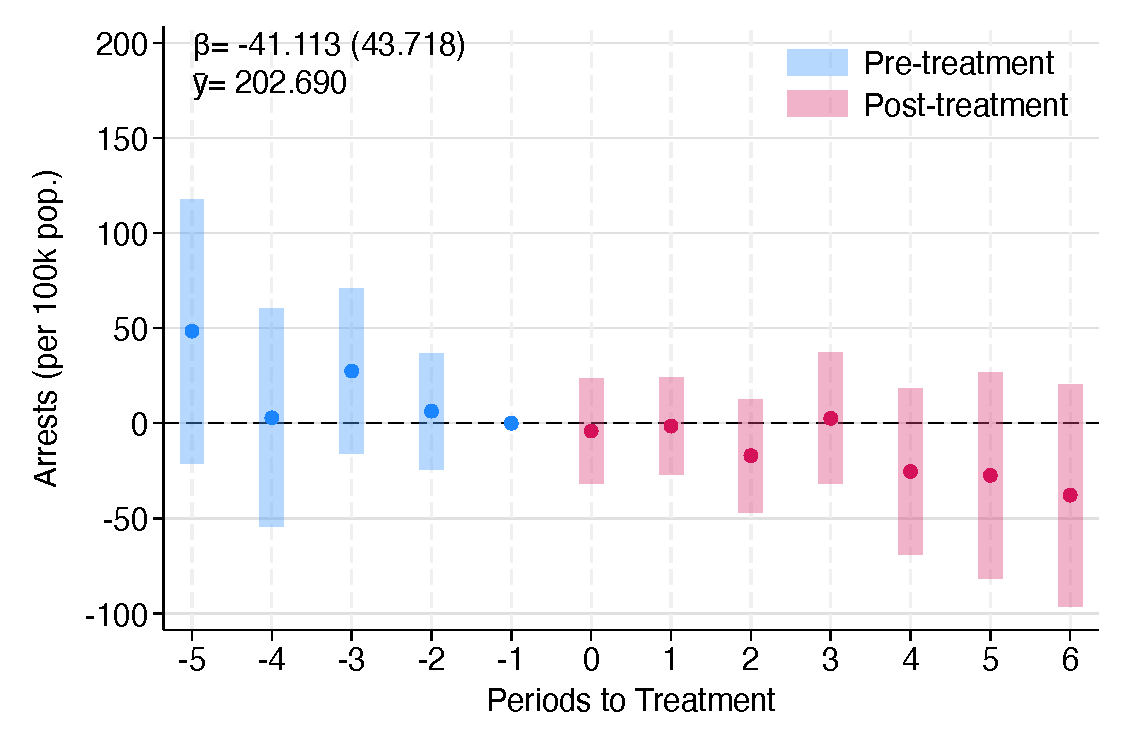
\includegraphics[width=0.98\textwidth]{../manuscript/Graphs/CHDH_continuous_spillover_arrests.pdf}
        \caption{Spillovers on Arrests}
    \end{subfigure}

    \vspace{0.5em}

    \begin{subfigure}{0.495\textwidth}
        \centering
        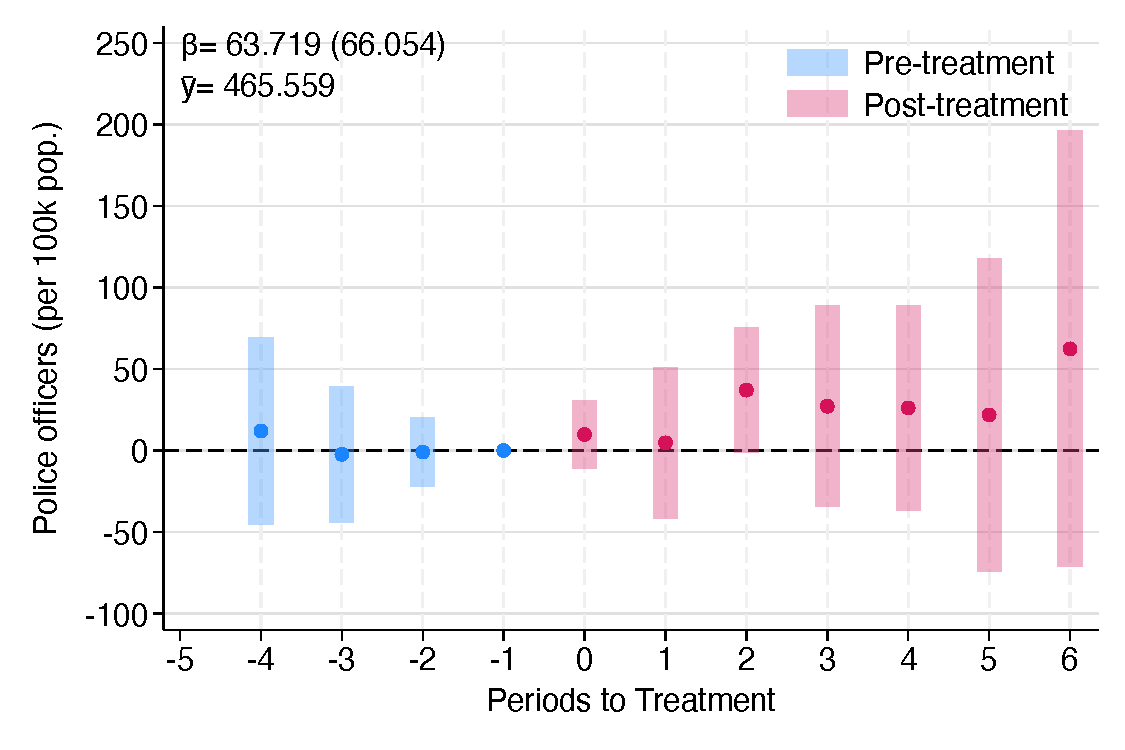
\includegraphics[width=0.98\textwidth]{../manuscript/Graphs/CHDH_continuous_spillover_dotpc.pdf}
        \caption{Spillovers on Police Officers}
    \end{subfigure}%
    ~
    \begin{subfigure}{0.495\textwidth}
        \centering
        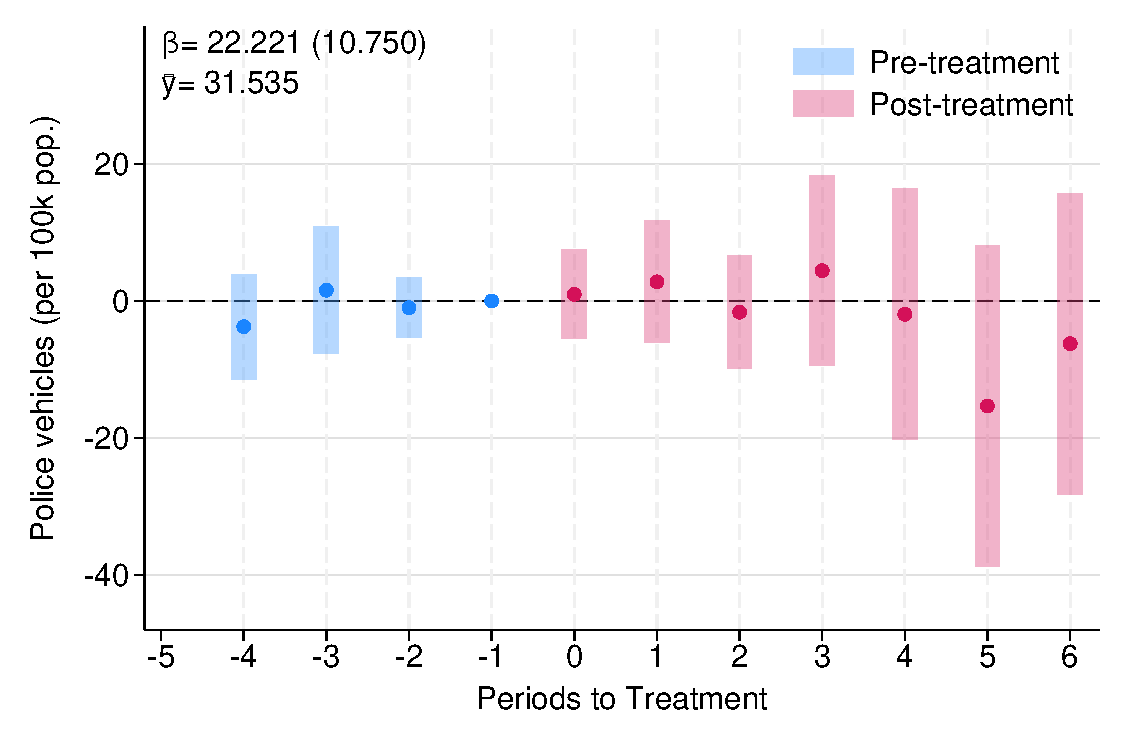
\includegraphics[width=0.98\textwidth]{../manuscript/Graphs/CHDH_continuous_spillover_vehiclespc.pdf}
        \caption{Spillovers on Patrol Vehicles}
    \end{subfigure}

    \begin{minipage}{0.95\textwidth}
    \footnotesize
    Notes: This figure reports the geographic spillover effects of \emph{Plan Cuadrante} on four outcomes for never-treated municipalities: reported crime per 100,000 inhabitants (panel a), arrests per 100,000 inhabitants (panel b), the number of police officers per 100,000 inhabitants (panel c), and the number of patrol vehicles per 100,000 inhabitants (panel d). Unlike the dummy spillover specification, the treatment variable is now continuous and equals the share of neighboring municipalities that have implemented \emph{Plan Cuadrante} by year $t$, following the spillover-intensity approach of \citet{crepon2013}. The sample is restricted to municipalities that never adopted \emph{Plan Cuadrante}. Estimation is performed using the heterogeneity-robust estimator of \citet{Chaisemartin}, which accommodates a continuous, time-varying treatment intensity in a staggered design. The dots represent the estimated dynamic effects and the bars behind them denote 95\% confidence intervals. Standard errors are clustered at the municipality level. The pooled effect  and the mean of the outcome among municipalities with no treated neighbors are reported in each panel.
    \end{minipage}
\end{figure}


\begin{figure}[h!]
    \centering
    \caption{Geographic Spillovers of \emph{Plan Cuadrante} by Number of Treated Neighbors}
    \label{fig:figure_count_spillovers}
    \begin{subfigure}{0.495\textwidth}
        \centering
        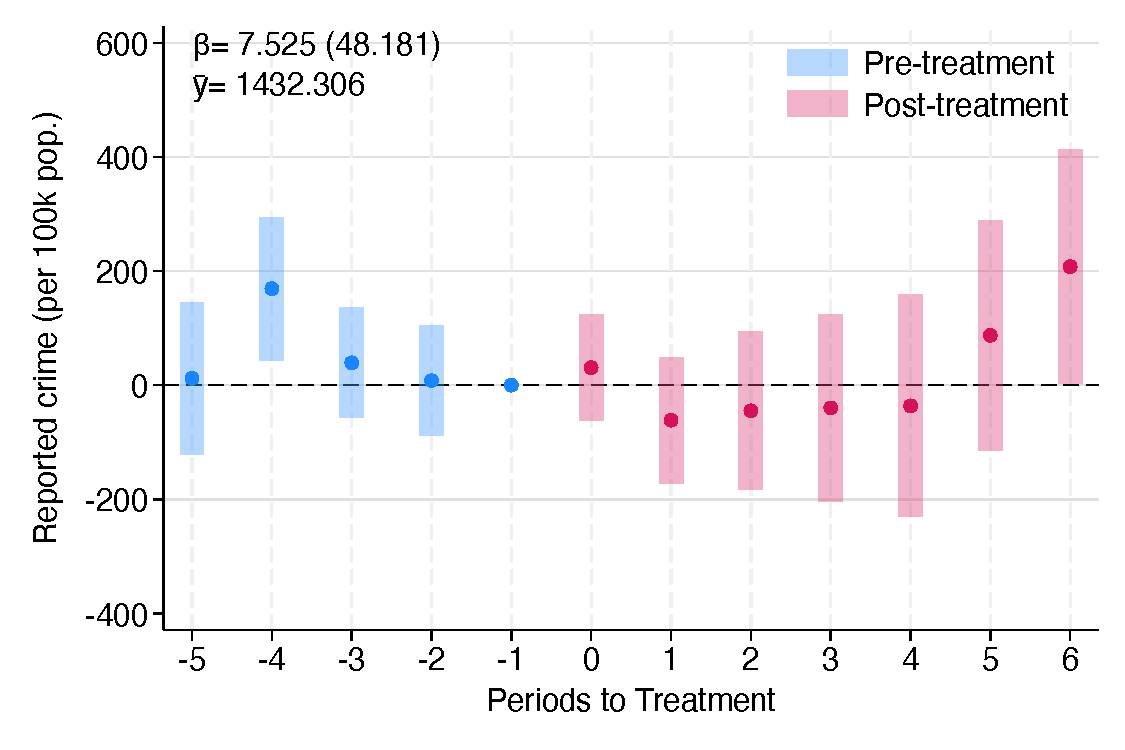
\includegraphics[width=0.98\textwidth]{../manuscript/Graphs/CHDH_continuous_spillover_crime_count.pdf}
        \caption{Spillovers on Reported Crime}
    \end{subfigure}%
    ~
    \begin{subfigure}{0.495\textwidth}
        \centering
        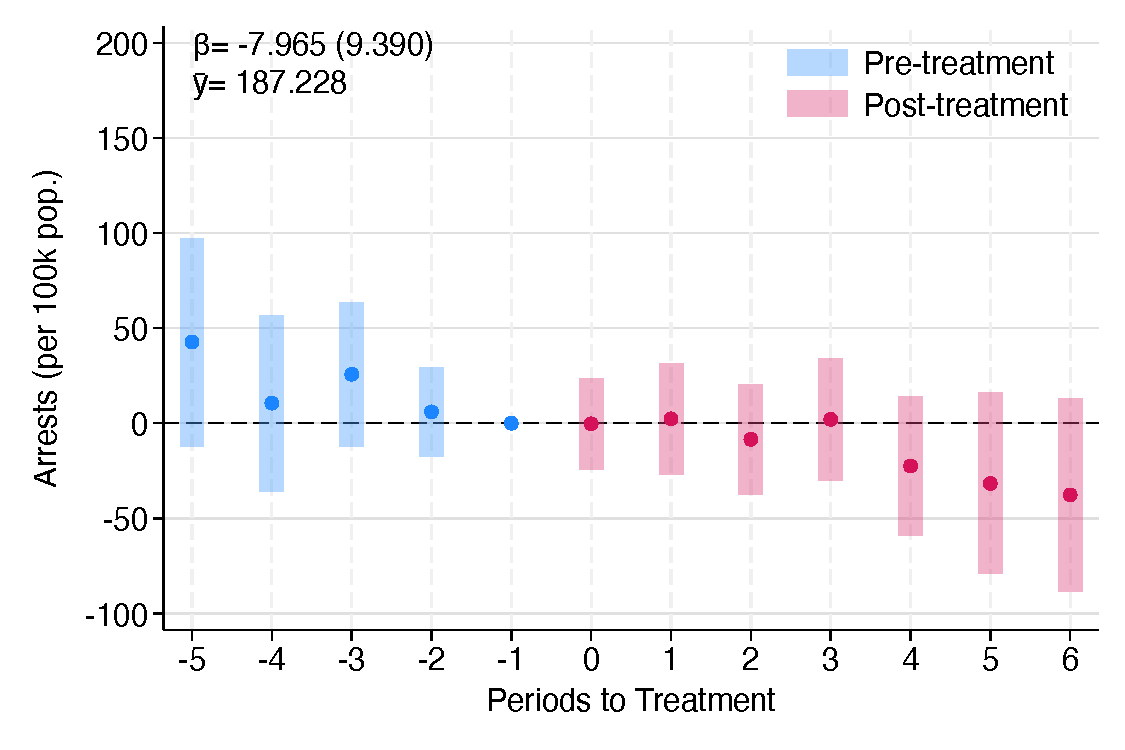
\includegraphics[width=0.98\textwidth]{../manuscript/Graphs/CHDH_continuous_spillover_arrests_count.pdf}
        \caption{Spillovers on Arrests}
    \end{subfigure}

    \vspace{0.5em}

    \begin{subfigure}{0.495\textwidth}
        \centering
        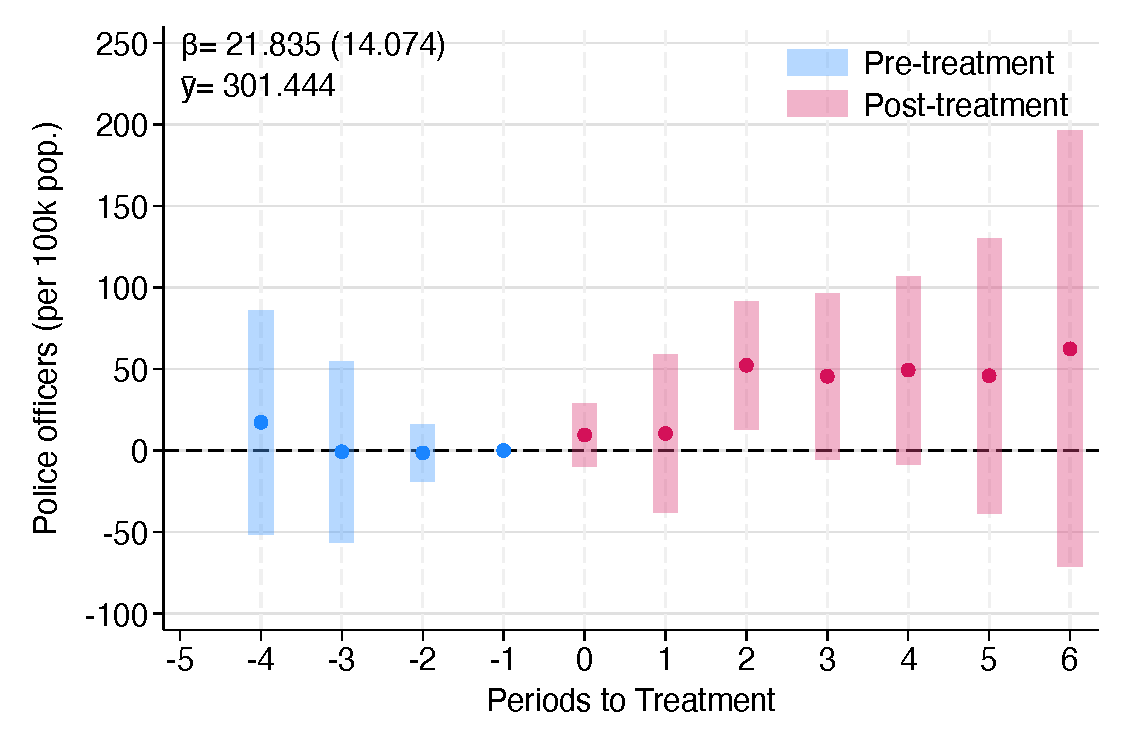
\includegraphics[width=0.98\textwidth]{../manuscript/Graphs/CHDH_continuous_spillover_dotpc_count.pdf}
        \caption{Spillovers on Police Officers}
    \end{subfigure}%
    ~
    \begin{subfigure}{0.495\textwidth}
        \centering
        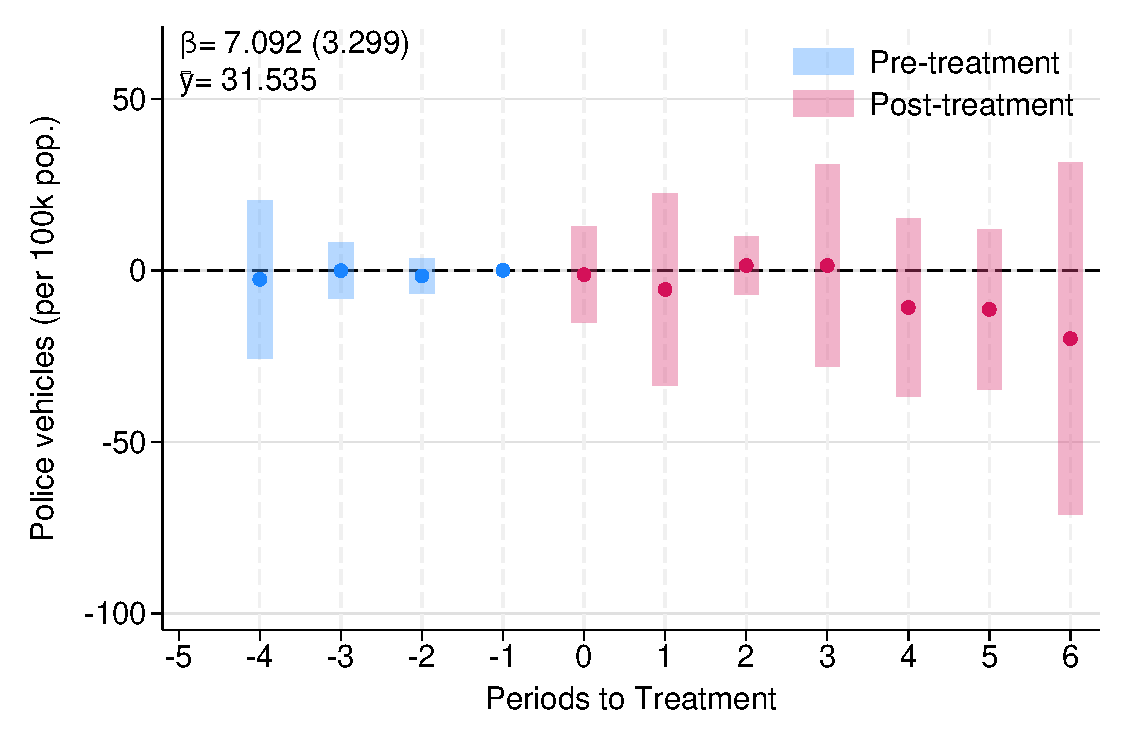
\includegraphics[width=0.98\textwidth]{../manuscript/Graphs/CHDH_continuous_spillover_vehiclespc_count.pdf}
        \caption{Spillovers on Patrol Vehicles}
    \end{subfigure}

    \begin{minipage}{0.95\textwidth}
    \footnotesize
    Notes: This figure reports the geographic spillover effects of \emph{Plan Cuadrante} on four outcomes for never-treated municipalities: reported crime per 100,000 inhabitants (panel a), arrests per 100,000 inhabitants (panel b), the number of police officers per 100,000 inhabitants (panel c), and the number of patrol vehicles per 100,000 inhabitants (panel d). Unlike the dummy spillover specification, the treatment variable is now continuous and equals the number of neighboring municipalities that have implemented \emph{Plan Cuadrante} by year $t$, following the spillover-intensity approach of \citet{crepon2013}. The sample is restricted to municipalities that never adopted \emph{Plan Cuadrante}. Estimation is performed using the heterogeneity-robust estimator of \citet{Chaisemartin}, which accommodates a continuous, time-varying treatment intensity in a staggered design. The dots represent the estimated dynamic effects and the bars behind them denote 95\% confidence intervals. Standard errors are clustered at the municipality level. The pooled effect  and the mean of the outcome among municipalities with no treated neighbors are reported in each panel.
    \end{minipage}
\end{figure}
}

\clearpage

{\renewcommand{\thefigure}{C.15}
\begin{figure}[h!]
    \centering
    \caption{Randomization Inference for the Direct and Spillover Effects of \emph{Plan Cuadrante}}
    \label{fig:ri_placebo}
    \begin{subfigure}{0.495\textwidth}
        \centering
        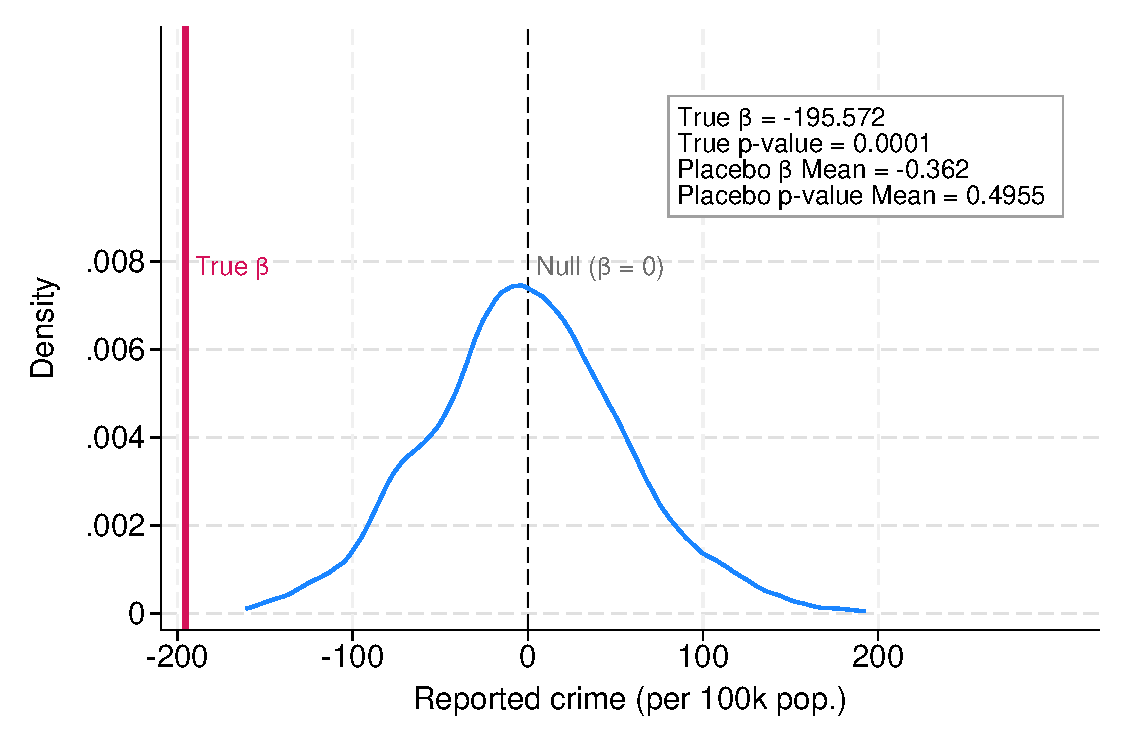
\includegraphics[width=\textwidth]{../manuscript/Graphs/CHDH_RI_placebo_crime.pdf}
        \caption{Reported crime}
        \label{fig:ri_crime}
    \end{subfigure}%
    ~
    \begin{subfigure}{0.495\textwidth}
        \centering
        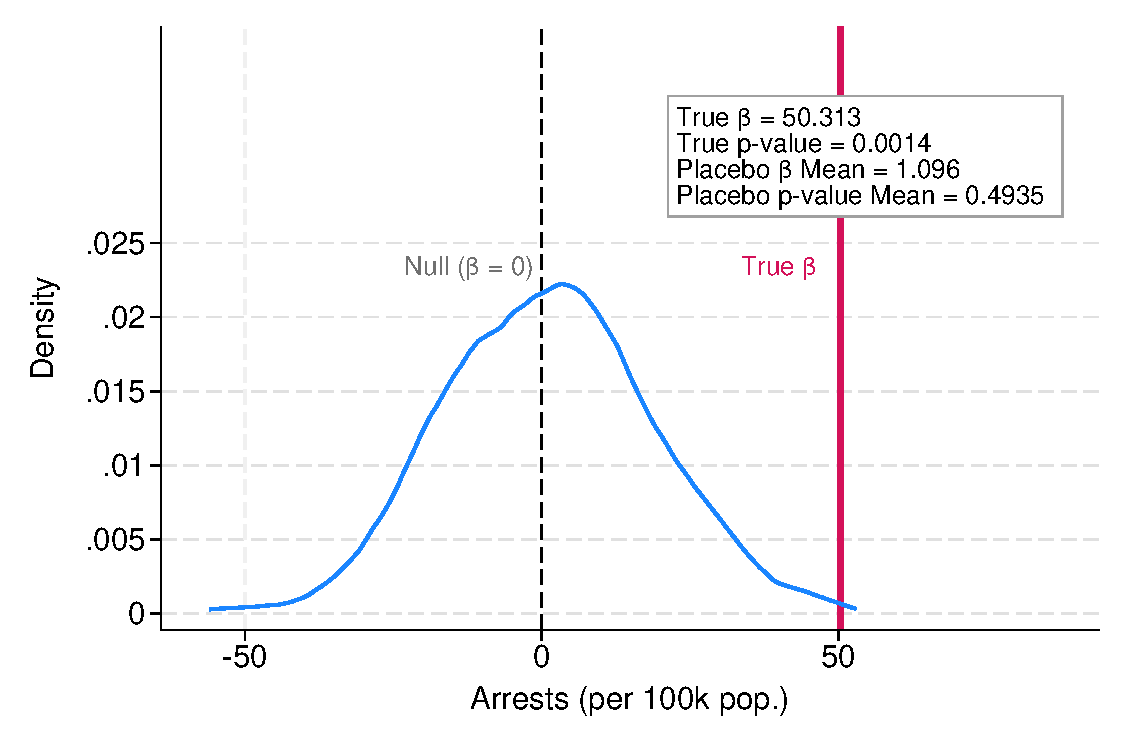
\includegraphics[width=\textwidth]{../manuscript/Graphs/CHDH_RI_placebo_arrests.pdf}
        \caption{Arrests}
        \label{fig:ri_arrests}
    \end{subfigure}

    \begin{subfigure}{0.495\textwidth}
        \centering
        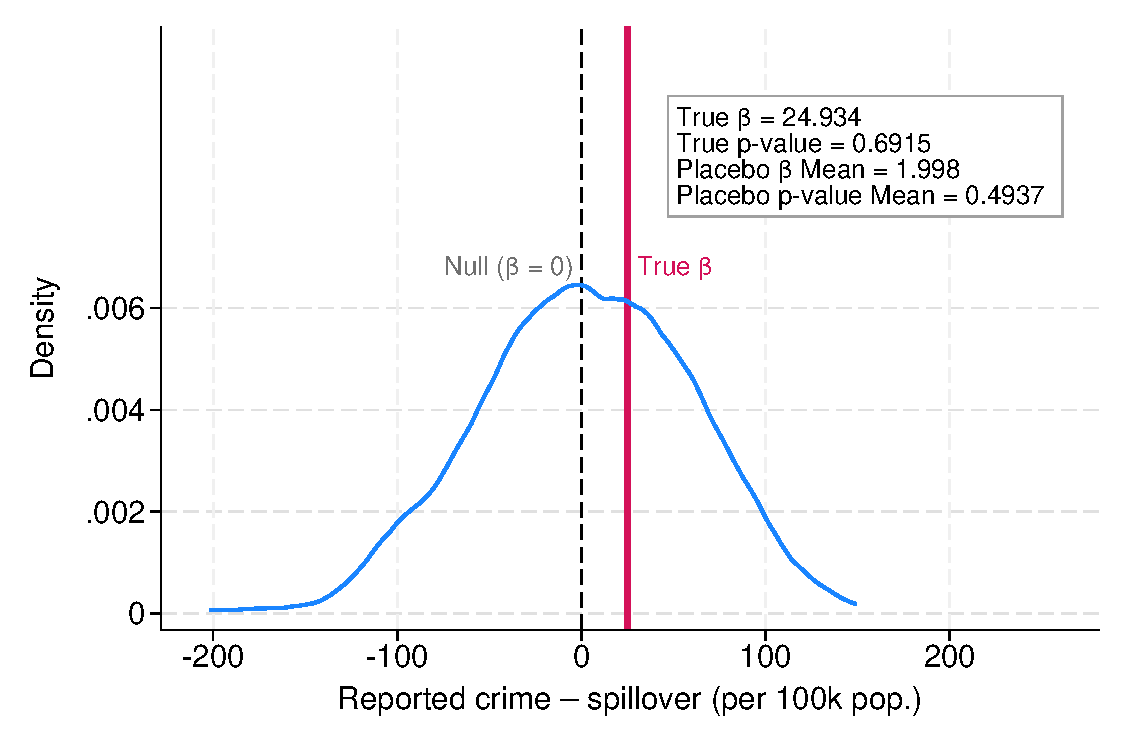
\includegraphics[width=\textwidth]{../manuscript/Graphs/CHDH_RI_placebo_crime_spillover.pdf}
        \caption{Spillovers on Reported crime}
        \label{fig:ri_crime_spillover}
    \end{subfigure}%
    \begin{subfigure}{0.495\textwidth}
        \centering
        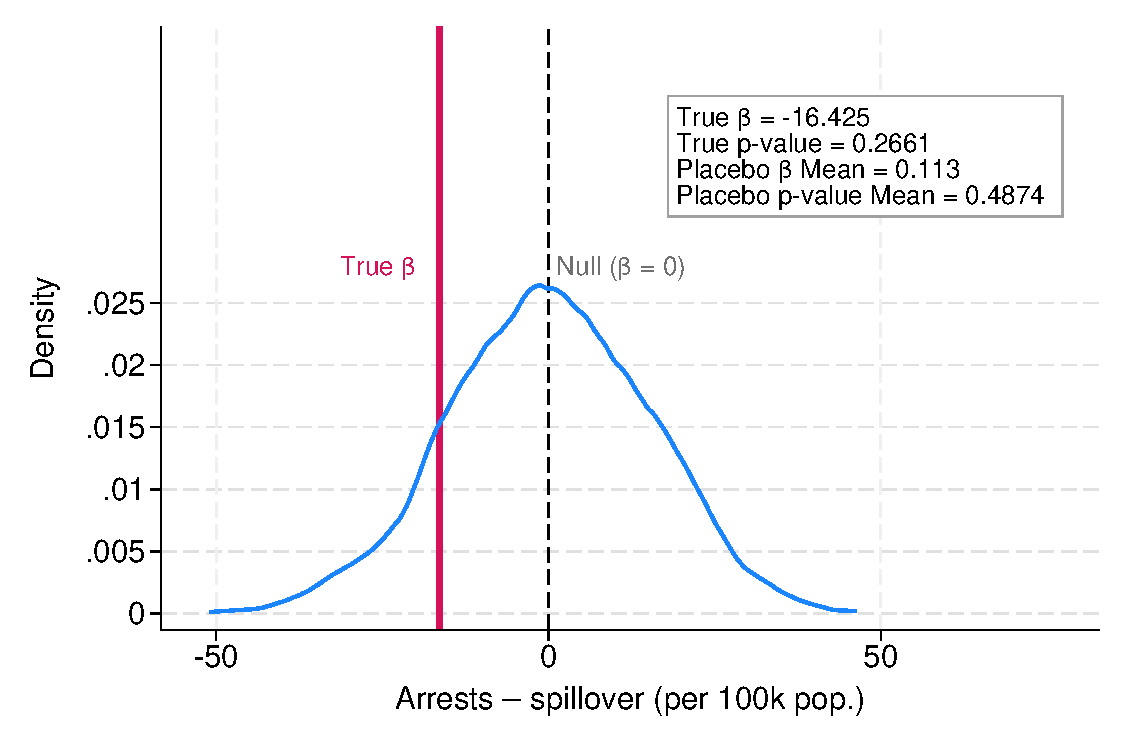
\includegraphics[width=\textwidth]{../manuscript/Graphs/CHDH_RI_placebo_arrests_spillover.pdf}
        \caption{Spillovers on Arrests}
        \label{fig:ri_arrests_spillover}
    \end{subfigure}
    \begin{minipage}{0.95\textwidth}
    \footnotesize
    Notes: This figure presents randomization inference results under the sharp null of no treatment effect, using the heterogeneity-robust estimator of \citet{Chaisemartin}. Each curve is the kernel density of 1{,}000 placebo ATT estimates obtained by jointly permuting \emph{Plan Cuadrante} adoption dates and never-treated status across municipalities (drawing from the empirical distribution of (date, status) pairs, so the marginal counts of treated and never-treated municipalities are preserved in every permutation). In each permutation the variable PC is shuffled across all 346 municipalities and a new time-varying treatment indicator is computed before re-estimating the dynamic effects. The solid colored vertical line marks the point estimate from the true rollout; the dashed black line marks the null expectation $\beta = 0$. The boxes report the true point estimate, its asymptotic two-sided $p$-value, and the mean of the placebo $\beta$ and placebo $p$-value distributions.
    \end{minipage}
\end{figure}
}

\clearpage

{\setcounter{figure}{15}\renewcommand{\thefigure}{C.\arabic{figure}}
\begin{figure}[h!]
    \centering
    \caption{Geographic Spillovers of \emph{Plan Cuadrante} for Neighbors of the ENUSC Municipalities (Administrative Outcomes)}
    \label{fig:figure_46ENUSC_spillovers_admin}
    \begin{subfigure}{0.495\textwidth}
        \centering
        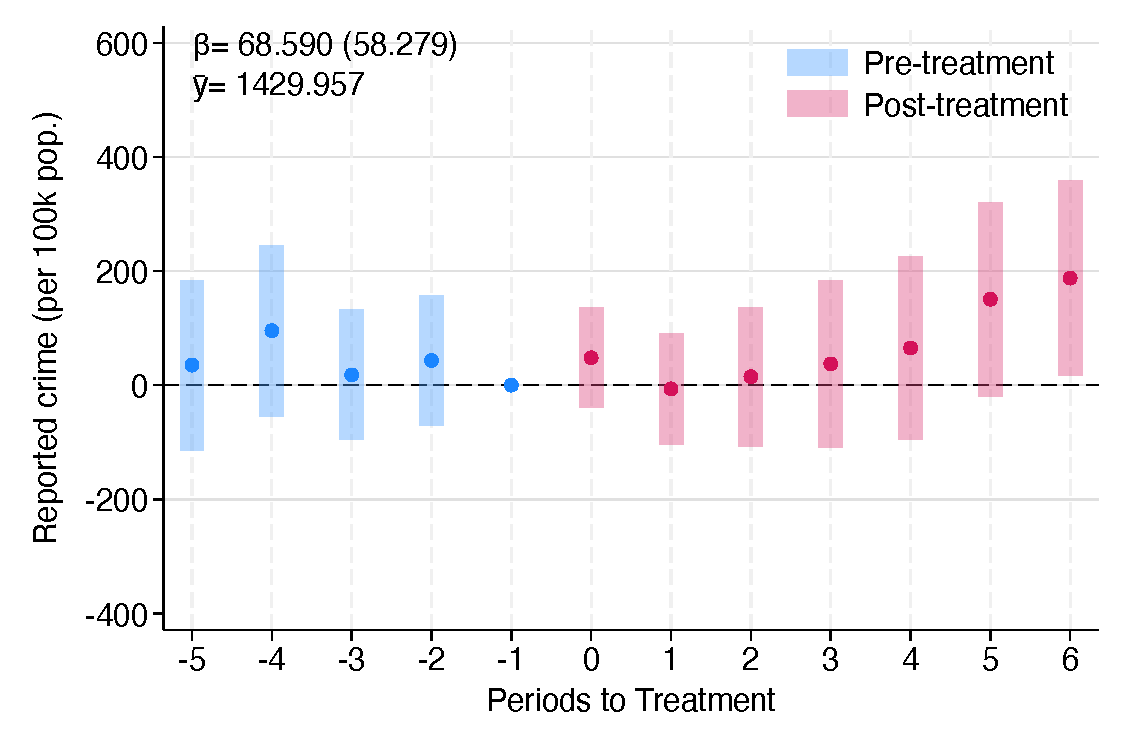
\includegraphics[width=0.98\textwidth]{../manuscript/Graphs/totalreportedcrime_enusc47_neighbors.pdf}
        \caption{Spillovers on Reported Crime}
    \end{subfigure}%
    ~
    \begin{subfigure}{0.495\textwidth}
        \centering
        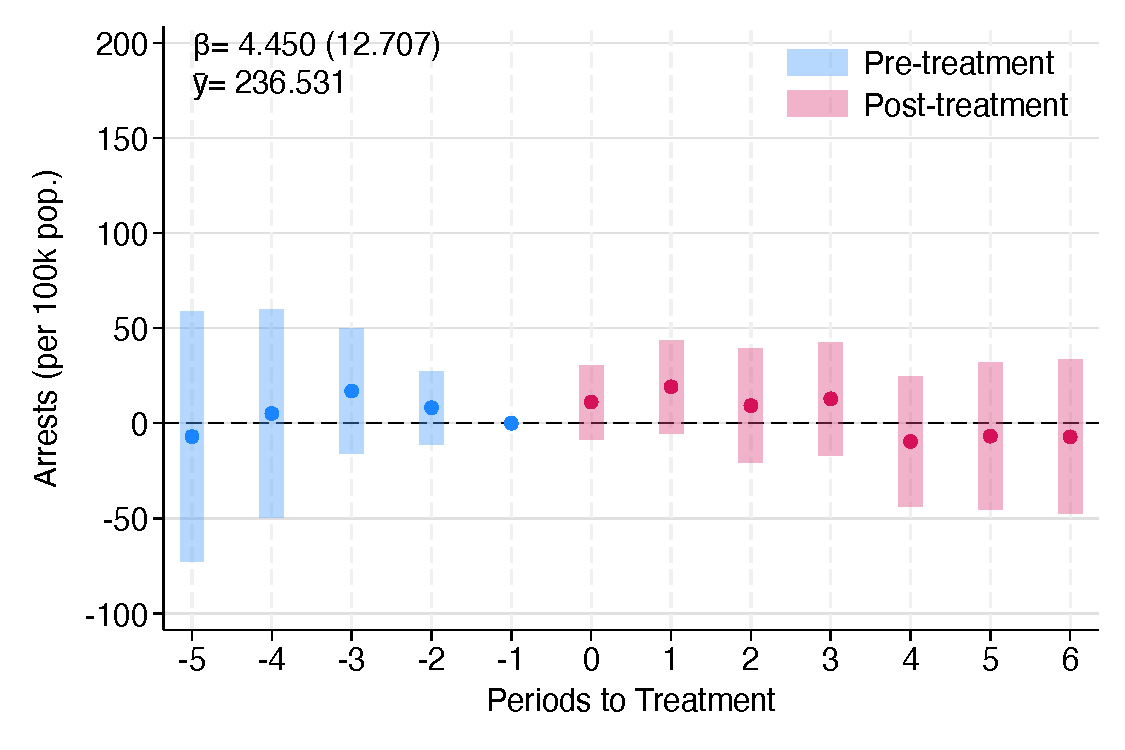
\includegraphics[width=0.98\textwidth]{../manuscript/Graphs/totalarrestscrime_enusc47_neighbors.pdf}
        \caption{Spillovers on Arrests}
    \end{subfigure}

    \vspace{0.5em}

    \begin{subfigure}{0.495\textwidth}
        \centering
        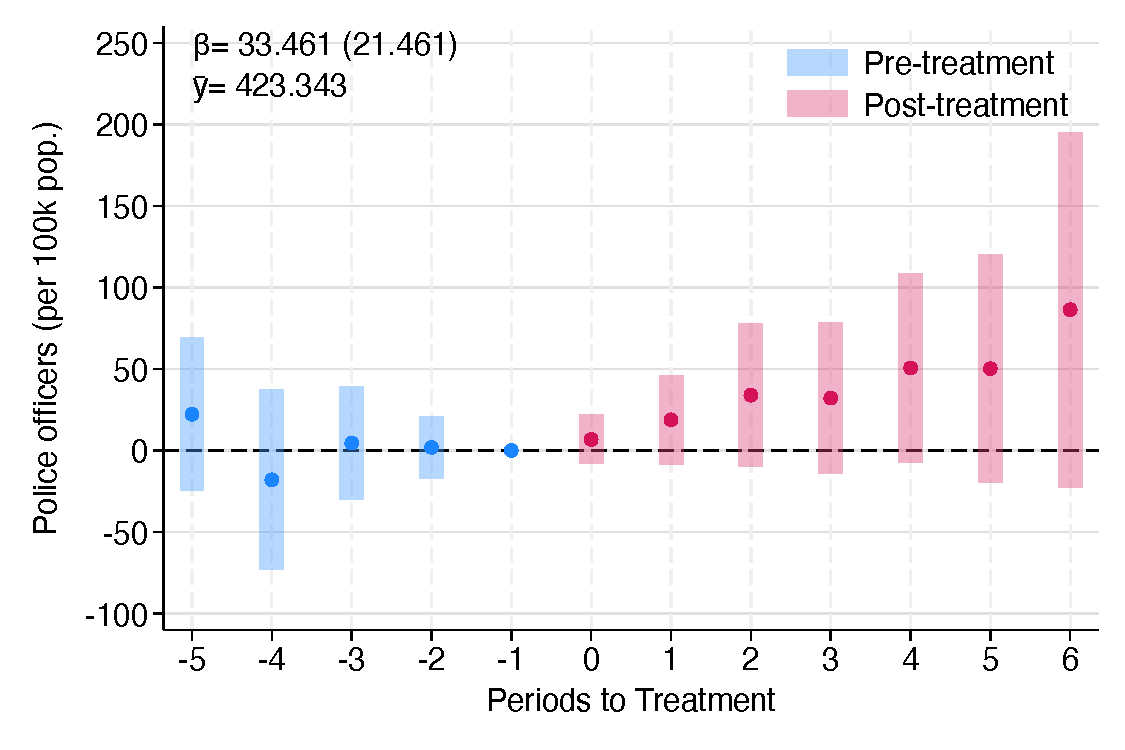
\includegraphics[width=0.98\textwidth]{../manuscript/Graphs/dotpc_enusc47_neighbors.pdf}
        \caption{Spillovers on Police Officers}
    \end{subfigure}%
    ~
    \begin{subfigure}{0.495\textwidth}
        \centering
        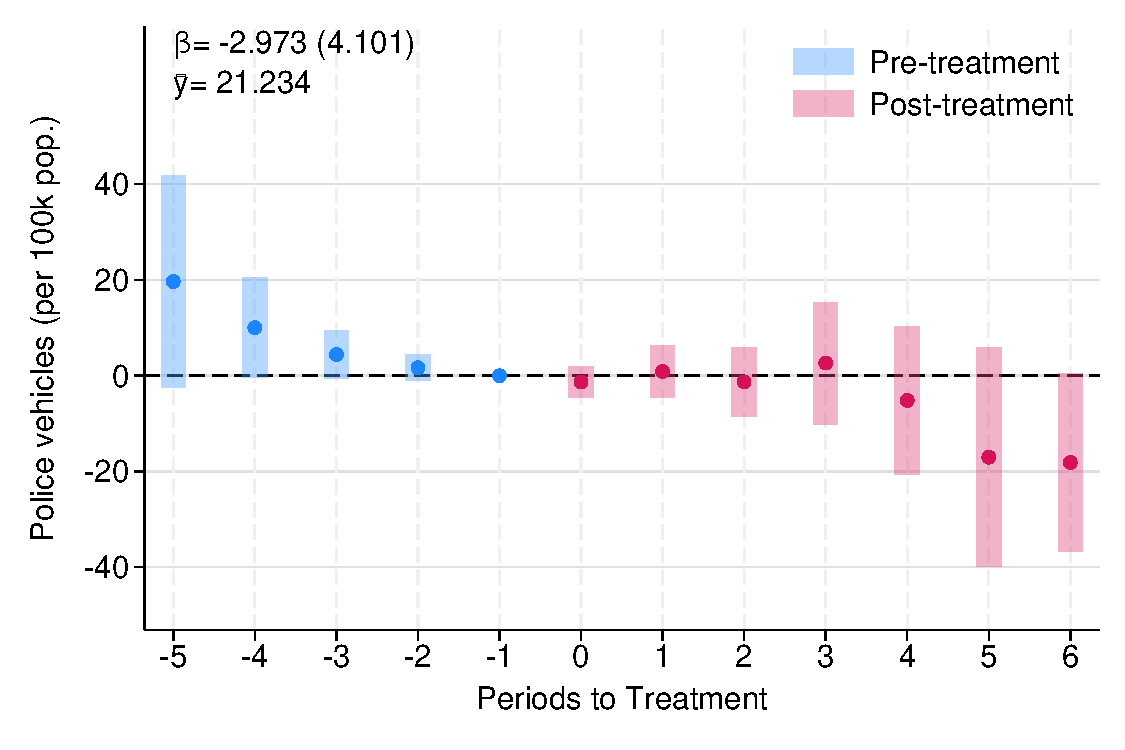
\includegraphics[width=0.98\textwidth]{../manuscript/Graphs/vehiclespc_enusc47_neighbors.pdf}
        \caption{Spillovers on Patrol Vehicles}
    \end{subfigure}

\begin{minipage}{\textwidth}
\footnotesize Notes: This figure reports the spillover effects of \emph{Plan Cuadrante} on the number of crimes reported to the police in the municipality per 100,000 inhabitants (panel a), on the number of arrests in the municipality per 100,000 inhabitants (panel b), on the number of police officers (panel c), and on the number of patrol vehicles (panel d). Specifically, the figure shows the dynamic effects of \emph{Plan Cuadrante} for neighboring never-treated municipalities to the 46 municipalities included in the ENUSC sample. The estimation is conducted using the procedure developed in \citet{Callaway} for difference-in-differences with staggered treatment adoption, using as the treatment introduction date the earliest date of a neighboring municipality. The dots in the figure represent the estimated coefficients and the bars behind them 95\% confidence intervals. Standard errors are clustered at the municipality level using the wild bootstrap procedure. The pooled effect and the mean outcome before the introduction of the treatment for each outcome are also presented in each panel.
\end{minipage}
\end{figure}


\begin{figure}[h!]
    \centering
    \caption{Geographic Spillovers of \emph{Plan Cuadrante} on ENUSC Survey Outcomes (Early- to Late-Adopting Municipalities)}
    \label{fig:figure_results_spillovers_enusc}
    \begin{subfigure}{0.495\textwidth}
        \centering
        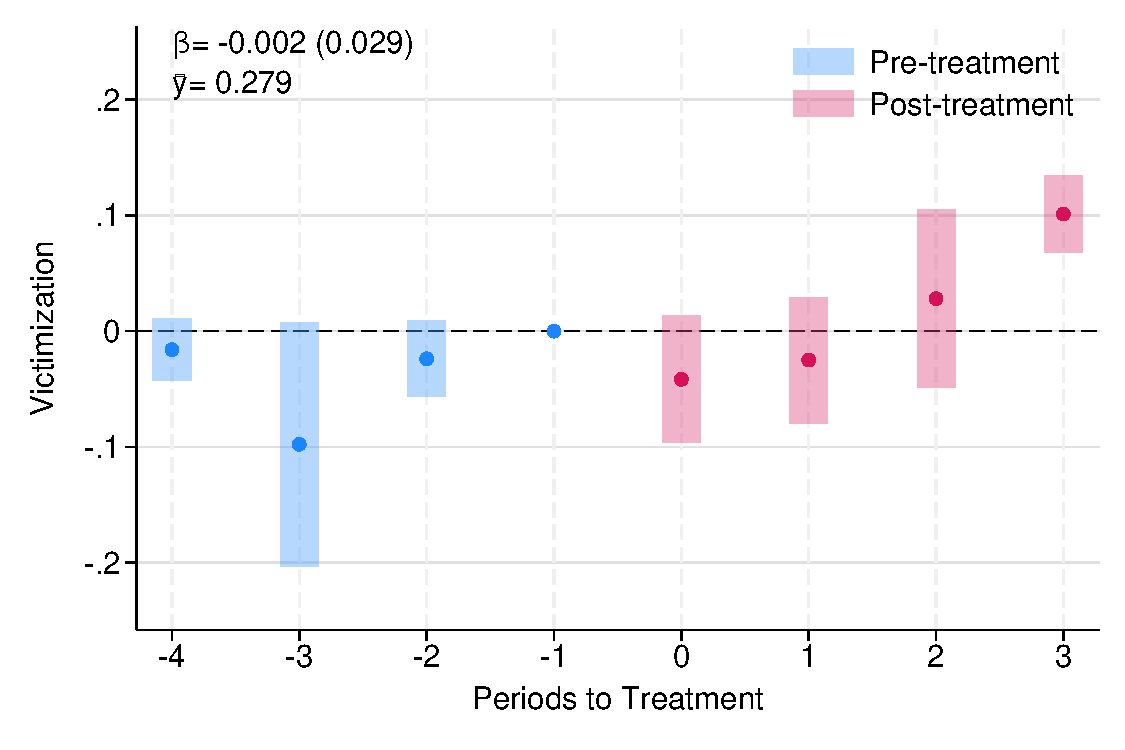
\includegraphics[width=0.98\textwidth]{../manuscript/Graphs/results_spillover_delitos.pdf}
        \caption{Spillovers on Victimization in last 12 months}
    \end{subfigure}%
    ~
    \begin{subfigure}{0.495\textwidth}
        \centering
        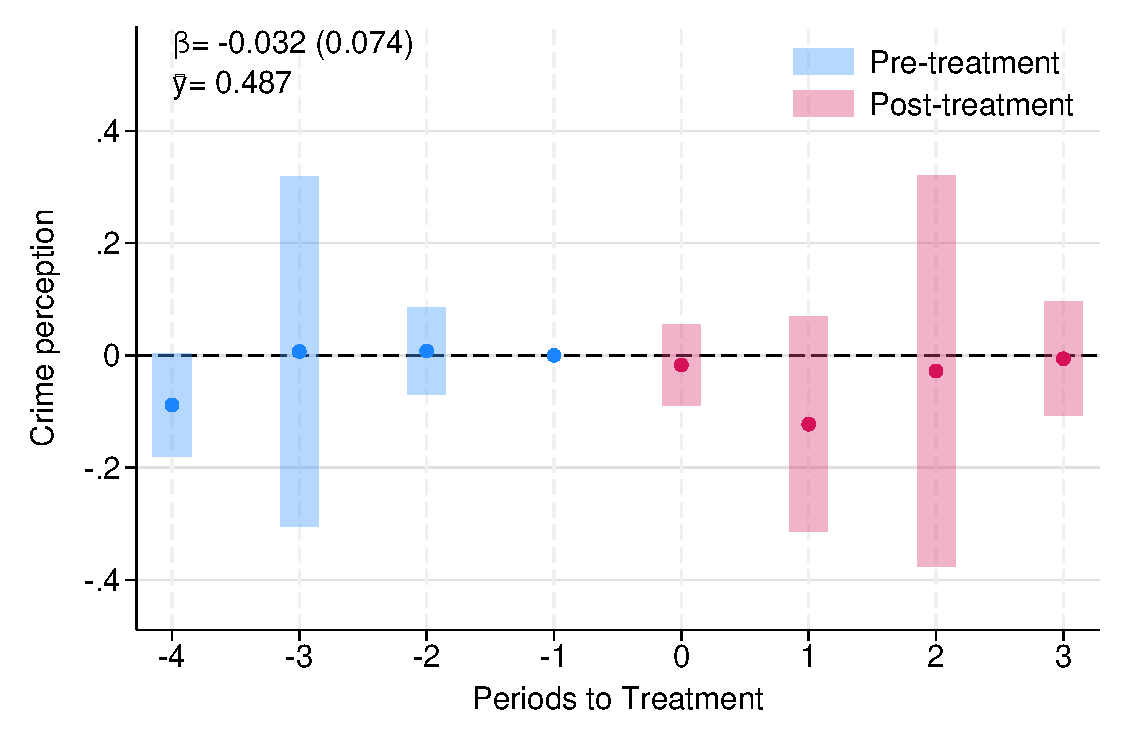
\includegraphics[width=0.98\textwidth]{../manuscript/Graphs/results_spillover_inseguridad_barrio1.pdf}
        \caption{Spillovers on Households reporting an increase in crime}
    \end{subfigure}
    \vspace{0.5em}
    \begin{subfigure}{0.495\textwidth}
        \centering
        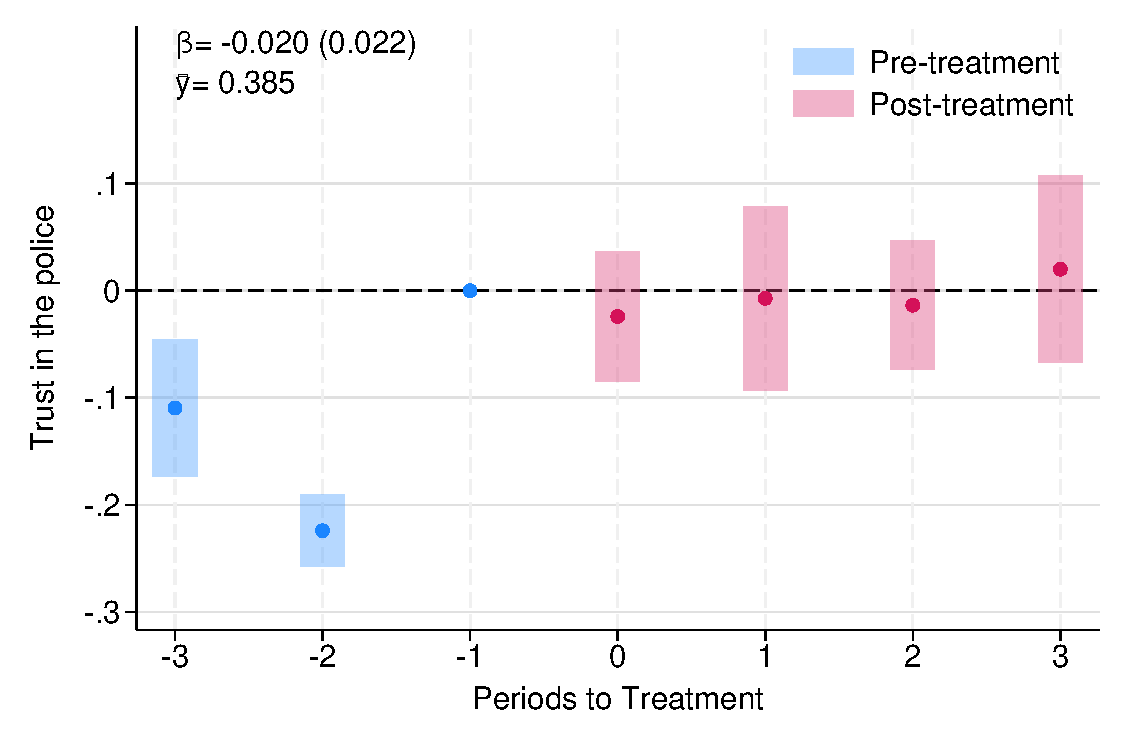
\includegraphics[width=0.98\textwidth]{../manuscript/Graphs/results_spillover_confianza_carabineros.pdf}
        \caption{Spillovers on Trust in the police}
    \end{subfigure}%
    ~
    \begin{subfigure}{0.495\textwidth}
        \centering
        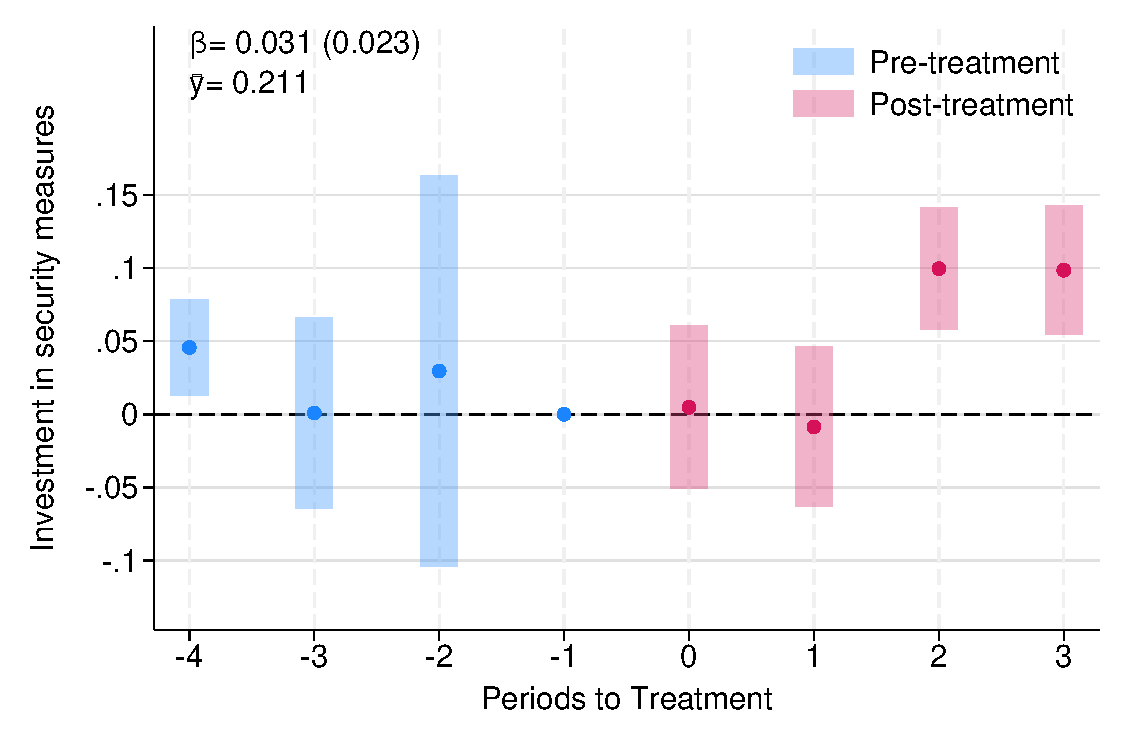
\includegraphics[width=0.98\textwidth]{../manuscript/Graphs/results_spillover_medidas_general_12.pdf}
        \caption{Spillovers on Households adopting security measures}
    \end{subfigure}
    \begin{minipage}{0.95\textwidth}
    \footnotesize
    Notes: This figure presents the geographic spillover effects of \emph{Plan Cuadrante} from early-adopting ENUSC municipalities on their late-adopting ENUSC neighbours, using the ENUSC sample. Panel (a) reports the effect of \emph{Plan Cuadrante} on the probability of household victimization in the last 12-months using the ENUSC survey. Panel (b) reports the effect on crime perception using the ENUSC survey. Panel (c) reports the effect on trust in the police using the ENUSC survey. Panel (d) reports the results on the probability of purchasing private security measures in the last twelve months using the ENUSC survey. The focal treated sample consists of six late-adopting ENUSC municipalities---Molina, Tocopilla, San Carlos, Padre Hurtado, Calera, and Limache---each assigned a spillover-onset date equal to the year its earliest-adopting ENUSC neighbour received \emph{Plan Cuadrante}: Curic\'o (2005) for Molina, Iquique (2005) for Tocopilla, Chill\'an (2007) for San Carlos, Pe\~naflor (2008) for Padre Hurtado, and Quillota (2008) for both Calera and Limache. Estimation is performed using the difference-in-differences estimator for staggered treatment adoption of \citet{Callaway}. The dots represent the estimated dynamic effects and the bars behind them denote 95\% confidence intervals. Standard errors are clustered at the municipality level. The pooled effect  and the mean of the outcome among municipalities with no treated neighbors are reported in each panel.
    \end{minipage}
\end{figure}

}

\clearpage

